%%%%%%%%%%%%%%%%%%%%%%%%%%%%%%%%%%%%%%%%%
% Arsclassica Article
% LaTeX Template
% Version 1.1 (10/6/14)
%
% This template has been downloaded from:
% http://www.LaTeXTemplates.com
%
% Original author:
% Lorenzo Pantieri (http://www.lorenzopantieri.net) with extensive modifications by:
% Vel (vel@latextemplates.com)
%
% License:
% CC BY-NC-SA 3.0 (http://creativecommons.org/licenses/by-nc-sa/3.0/)
%
%%%%%%%%%%%%%%%%%%%%%%%%%%%%%%%%%%%%%%%%%

%----------------------------------------------------------------------------------------
%	PACKAGES AND OTHER DOCUMENT CONFIGURATIONS
%----------------------------------------------------------------------------------------

\documentclass[
10pt, % Main document font size
a4paper, % Paper type, use 'letterpaper' for US Letter paper
oneside, % One page layout (no page indentation)
%twoside, % Two page layout (page indentation for binding and different headers)
headinclude,footinclude, % Extra spacing for the header and footer
BCOR5mm, % Binding correction
]{scrartcl}

%%%%%%%%%%%%%%%%%%%%%%%%%%%%%%%%%%%%%%%%%
% Arsclassica Article
% Structure Specification File
%
% This file has been downloaded from:
% http://www.LaTeXTemplates.com
%
% Original author:
% Lorenzo Pantieri (http://www.lorenzopantieri.net) with extensive modifications by:
% Vel (vel@latextemplates.com)
%
% License:
% CC BY-NC-SA 3.0 (http://creativecommons.org/licenses/by-nc-sa/3.0/)
%
%%%%%%%%%%%%%%%%%%%%%%%%%%%%%%%%%%%%%%%%%

%----------------------------------------------------------------------------------------
%	REQUIRED PACKAGES
%----------------------------------------------------------------------------------------

\usepackage[
nochapters, % Turn off chapters since this is an article        
beramono, % Use the Bera Mono font for monospaced text (\texttt)
eulermath,% Use the Euler font for mathematics
pdfspacing, % Makes use of pdftex’ letter spacing capabilities via the microtype package
dottedtoc % Dotted lines leading to the page numbers in the table of contents
]{classicthesis} % The layout is based on the Classic Thesis style

\usepackage{arsclassica} % Modifies the Classic Thesis package

\usepackage[T1]{fontenc} % Use 8-bit encoding that has 256 glyphs

\usepackage[utf8]{inputenc} % Required for including letters with accents

\usepackage{graphicx} % Required for including images
\graphicspath{{Figures/}} % Set the default folder for images

\usepackage{enumitem} % Required for manipulating the whitespace between and within lists

\usepackage{lipsum} % Used for inserting dummy 'Lorem ipsum' text into the template

\usepackage{subfig} % Required for creating figures with multiple parts (subfigures)

\usepackage{amsmath,amssymb,amsthm} % For including math equations, theorems, symbols, etc

\usepackage{varioref} % More descriptive referencing

%----------------------------------------------------------------------------------------
%	THEOREM STYLES
%---------------------------------------------------------------------------------------

\theoremstyle{definition} % Define theorem styles here based on the definition style (used for definitions and examples)
\newtheorem{definition}{Definition}

\theoremstyle{plain} % Define theorem styles here based on the plain style (used for theorems, lemmas, propositions)
\newtheorem{theorem}{Theorem}

\theoremstyle{remark} % Define theorem styles here based on the remark style (used for remarks and notes)

%----------------------------------------------------------------------------------------
%	HYPERLINKS
%---------------------------------------------------------------------------------------

\hypersetup{
%draft, % Uncomment to remove all links (useful for printing in black and white)
colorlinks=true, breaklinks=true, bookmarks=true,bookmarksnumbered,
urlcolor=webbrown, linkcolor=RoyalBlue, citecolor=webgreen, % Link colors
pdftitle={}, % PDF title
pdfauthor={\textcopyright}, % PDF Author
pdfsubject={}, % PDF Subject
pdfkeywords={}, % PDF Keywords
pdfcreator={pdfLaTeX}, % PDF Creator
pdfproducer={LaTeX with hyperref and ClassicThesis} % PDF producer
} % Include the structure.tex file which specified the document structure and layout

\hyphenation{Fortran hy-phen-ation} % Specify custom hyphenation points in words with dashes where you would like hyphenation to occur, or alternatively, don't put any dashes in a word to stop hyphenation altogether

%by nicu:
\newcommand\TODO[1]{\textcolor{red}{#1}}
\usepackage{chngpage}
\usepackage{tabularx}
\usepackage{pbox}
\usepackage{float}
\restylefloat{table}

\usepackage{graphicx}
\usepackage{wrapfig}
\usepackage{lscape}
\usepackage{rotating}
\usepackage{epstopdf}


%----------------------------------------------------------------------------------------
%	TITLE AND AUTHOR(S)
%----------------------------------------------------------------------------------------

\title{\normalfont\spacedallcaps{ASL Milestone 1}} % The article title

\author{\spacedlowsmallcaps{Niculin Tschurr\textsuperscript{1}}} % The article author(s) - author affiliations need to be specified in the AUTHOR AFFILIATIONS block

\date{} % An optional date to appear under the author(s)

%----------------------------------------------------------------------------------------

\begin{document}

%----------------------------------------------------------------------------------------
%	HEADERS
%----------------------------------------------------------------------------------------

\renewcommand{\sectionmark}[1]{\markright{\spacedlowsmallcaps{#1}}} % The header for all pages (oneside) or for even pages (twoside)
%\renewcommand{\subsectionmark}[1]{\markright{\thesubsection~#1}} % Uncomment when using the twoside option - this modifies the header on odd pages
\lehead{\mbox{\llap{\small\thepage\kern1em\color{halfgray} \vline}\color{halfgray}\hspace{0.5em}\rightmark\hfil}} % The header style

\pagestyle{scrheadings} % Enable the headers specified in this block

%----------------------------------------------------------------------------------------
%	TABLE OF CONTENTS & LISTS OF FIGURES AND TABLES
%----------------------------------------------------------------------------------------

\maketitle % Print the title/author/date block

\setcounter{tocdepth}{2} % Set the depth of the table of contents to show sections and subsections only

\tableofcontents % Print the table of contents

%\listoffigures % Print the list of figures

%\listoftables % Print the list of tables

%----------------------------------------------------------------------------------------
%	ABSTRACT
%----------------------------------------------------------------------------------------

\section*{Abstract} 
\TODO{write abstract}

%----------------------------------------------------------------------------------------
%	AUTHOR AFFILIATIONS
%----------------------------------------------------------------------------------------

{\let\thefootnote\relax\footnotetext{* \textit{tschurrn@student.ethz.ch}}}



%----------------------------------------------------------------------------------------

\newpage % Start the article content on the second page, remove this if you have a longer abstract that goes onto the second page

%----------------------------------------------------------------------------------------
%	INTRODUCTION
%----------------------------------------------------------------------------------------
\section{Introduction}
For the course Advanced Systems Lab I implemented a message passing system. In the following report, the system as well as design choices are explained. Some of the design decisions have been influenced by the way I originaly intended to test the system. The benefits and drawbacks of these decisions are discussed focussing on possible real world system as well as the performance during the tests that have been done on Amazon servers.



\section{Implementation}
This section first gives an overview of the system's components and how they work together. Afterwards the single components are discussed in more detail. 

\subsection{Overall design}
The application consists of three major components:
\begin{itemize}
	\item Database
	\item Middleware
	\item Client
\end{itemize}

Each component may run on a different machine and can be connected to another component via its IP address. There may only be one database, but as many clients and middlewares as wanted. My application requires every client to connect to a single middleware. This is sufficient for my application, since I can assume that the middlewares keep running during the whole time period of every test. All middlewares are connected to the same single database. In order to be able to simulate many clients on a single Amazon server instance a \texttt{ClientMaster} instance can create, register and deregister any number of clients. This has been implemented in order to facilitate creating database dumps and running experiments. The clients and middleware are implemented in two different Java projects. 


\begin{figure}[h]
\centering 
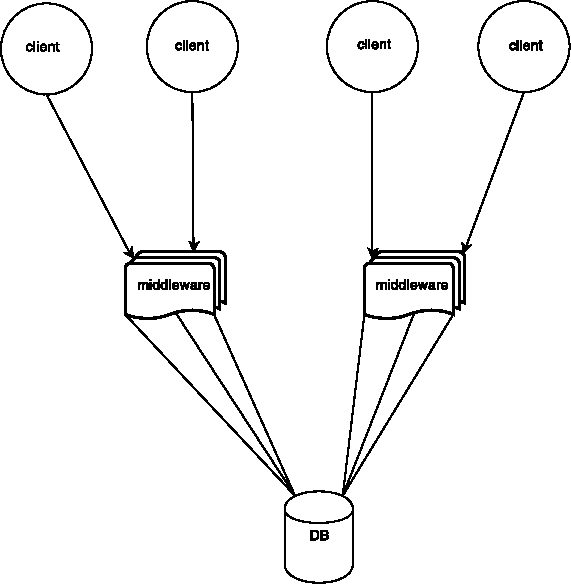
\includegraphics[scale=0.6]{overallDesign} 
\caption{Connections Overview} % The text in the square bracket is the caption for the list of figures while the text in the curly brackets is the figure caption
%\label{fig:gallery} 
\end{figure}


\subsection{Database}
This section gives an overview about the database implementation. Performance characteristics are discussed later with the other test results.

\subsubsection{Design}
The database needs to store all communication between the clients. Clients have to write messages into queues. Every message has to be in exactly one queue, but can be addressed to a specific receiver or to everyone. This is shown in the ER-diagramm with two different relations. A Client can decide wether to read or pop a message. In my system when a client reads a message that was specifically for it, the message is always deleted (no read specific receiver messages). I did this in order to shorten the livetime of these messages in the system. I also thought that when a message is for everyone, maybe more than one client may be interested in the message, but if it is for one specific client, the client is responsible for storing the message locally. 

\begin{figure}[h]
\centering
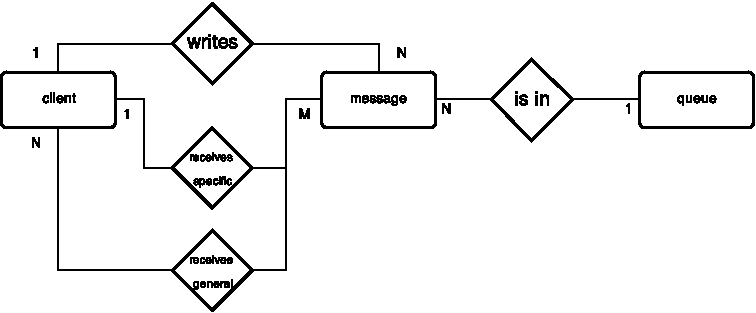
\includegraphics[scale=0.8]{er}
\caption{ER-diagramm}
\end{figure}


The database consists of 4 tables as shown below. I decided to create two tables to store all the information about a message. One table holds the message's content and an identifier, the other table holds all the needed metadata about the messages. By doing so, the metadata table has as many entries as when the content would be stored in the same table, but it needs much less memory. This design leads to many joins during runtime but on the other hand, I have many queries that only need the metadata table and then may read smaller tuples because the content is stored seperately. Overall I expect the cost of the joins to be bigger than what I save with the queries that only need the metadata table. I expect this especially because I added indices to every column in the metadata table. Therefore most queries perform the computationally intensive part only on the indices and then need to read only few tuples. The indices are required because there is a query for each column that needs to filter or sort it. The messages table references the metadata's primary key. This means that the message content has to be deleted before the metadata entry may be deleted. The table \texttt{queues} is required because a queue is not represented in the metadata table if it is empty. This may happen because all messages are deleted during runtime or when a new queue is created. By having an extra table where all the queues are stored the clients can easily find out in which queues they may write. The queues are referenced by the metadata table because in my system queues may be deleted only if a queue is empty. When a client tries to delete a non empty queue, it will fail because of the foreign key constraint.
Finally the table clients serves several purposes. It is also referenced by the metadata table. It therefore is not possible to write to a non existing client and creating messages which would never be read. The table \texttt{clients} is also used for the client's registration. Clients can not only be created but also deregisterd and afterwards re-registered. When a client is created an entry in the table is created. The column flag indicates if the client is currently registered.


\begin{table}[H]
\begin{adjustwidth}{-2in}{-2in}
\caption{Database Tables}
\centering
\begin{tabular}{|l|lll|l|}
\toprule
Table&
\multicolumn{3}{c|}{Columns} & Index \\
\cmidrule(l){2-4}
Name & Name & Type & Constraints & \\
\midrule
metadata & message\_id	& SERIAL & PRIMARY\_KEY & implicit\\
		&timestamp & timestamp & DEFAULT\_NOW() & Yes\\
			&queue\_id	&int 	& REFERENCES queues(queue\_id)&Yes\\
			&sender\_id	&int 	& REFERNCES clients(client\_id)&Yes\\
			&receiver\_id&int 	& REFERENCES clients(client\_id)& Yes\\
\midrule
messages	&message\_id&int 	& REFERENCES metadata(message\_id)&Yes\\
			&payload	&varchar(3000)& &No\\
\midrule
queues		&queue\_id 	&SERIAL & PRIMARY\_KEY&implicit\\
\midrule
clients 	&client\_id 	&SERIAL	& PRIMARY\_KEY&implicit\\
			&flag 		&boolean&DEFAULT TRUE&No\\
\bottomrule
\end{tabular}
\label{tab:db}
\end{adjustwidth}

\end{table}




\subsubsection{Initialization}
The database is initialazed with the tables and indices as indicated in the table \vref{tab:db}. Additionally a client with \texttt{client\_id} 0 is added. When a message is not intended for a specific client it is sent to \\texttt{client\_id} 0. When a client tries to read a message it filters for its own id or 0 as the receiver.

\subsubsection{Queries}
All queries are implemented as \texttt{PreparedStatement}. This speeds up query execution. An overview of the queries is given in table \vref{tab:queries}, for the queries themselves please have a look at the class \texttt{\textbackslash code\textbackslash middleware \textbackslash src\textbackslash middleware\textbackslash Queries.java}. The query \texttt{deleteQueue} could have been implemented to first check if the queue is empty and then return if the deletion was successful. Because of the foreign key constraint this is not required, since the query will simply fail if the queue isn't empty. 

\begin{table}[H]
\begin{adjustwidth}{-2in}{-2in}
\caption{Queries}
\centering
\begin{tabular}{|l|p{2cm}|p{2cm}|p{8cm}|}
\toprule
Name & Arguments &Return Values& Description\\
\midrule
\texttt{regNewCl} & -&new client\_id&a new client is created\\
\midrule
\texttt{regOldCl} & client\_id&-&sets the clients flag to \texttt{true}\\
\midrule
\texttt{deRegCl}&client\_id&-&sets the clients flag to \texttt{false}\\
\midrule
\texttt{createNewQueue}&-&queue\_id&creates a new queue\\
\midrule
\texttt{deleteQueue}&queue\_id&-&deletes the specified queue (only works if the queue is empty)\\
\midrule
\texttt{getClientIds}&-&client\_id&returns all active clients\\
\midrule
\texttt{getAllQueues}&-&queue\_id&returns all queues\\
\midrule
\texttt{getQueuesForClient}&\raggedright client\_id&queue\_id&get all queues where messages for the specified clients are\\
\midrule
\texttt{readTopMost}&\raggedright queue\_id, receiver\_id&payload&returns the topmost message from the specified queue that may be read by the client, meaning its addressed to it or to everybody\\
\midrule
\texttt{pop}&\raggedright queue\_id, receiver\_id&payload&same as \texttt{readTopMost}, but deletes the message before returning it\\
\midrule
\texttt{popFromOther}&\raggedright receiver\_id, sender\_id&payload&returns and deletes the oldest message that the specified sender sent to this specific receiver\\
\midrule
\texttt{insertMessage} & \raggedright queue\_id, sender\_id, receiver\_id, content & - &creates a message in the metadata table in the given queue with the specified sender and receiver, the content stored in the \texttt{messages} table \\
\bottomrule
\end{tabular}
\label{tab:queries}
\end{adjustwidth}

\end{table}



\subsection{Middleware}
This section describes the middleware which communicates between the database and the clients. It focuses on the implementation. The performance characteristics are discussed later. Many clients can be connected to the middleware over a single port and the middleware has several connections to the database. Figure \vref{fig:middleware} shows the overall design of the middleware. 

\begin{figure}[H]
\centering
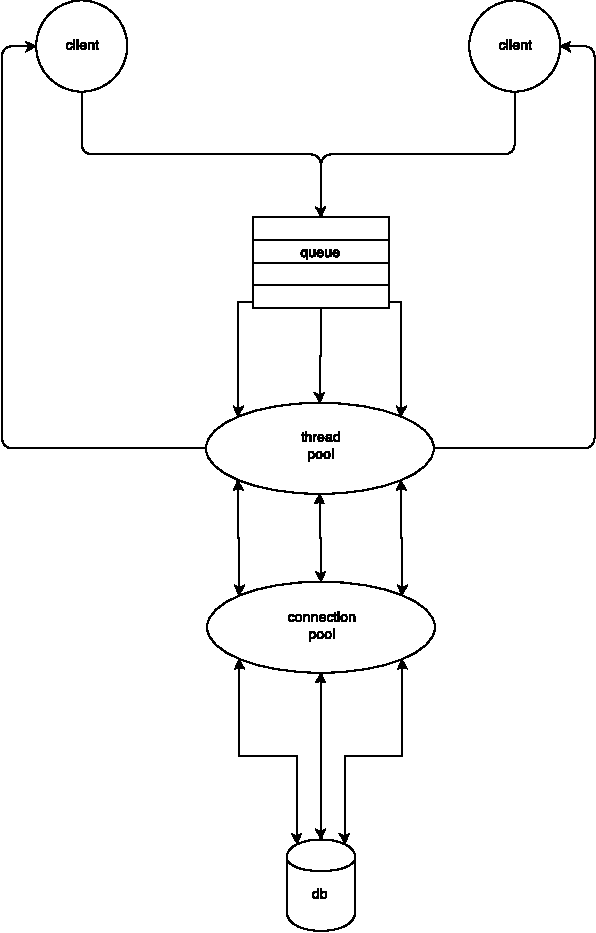
\includegraphics[scale=0.8]{middleware}
\caption{Middleware Design}
\label{fig:middleware}
\end{figure}

The class \texttt{Controller} initializes the middleware by creating a thread that listens to incomming messages from clients, a thread pool that handles the client's requests, a database connection pool that is used by the handler threads and finally a logger. 
A client can connect to the middleware with its IP address on port 9000. The middleware runs a thread \texttt{RequestAcceptor} which queues all the client requests. 
The threads that execute the client requests are implemented in a thread pool. Everytime a thread from this pool finishes a request, the \texttt{RequestAcceptor} assigns it a new one.
The thread handles the client request, which means it queries the database and returns the result to the client. This is implemented in the class\texttt{Handler}. This class first reads the clients socket and parses the request. It then attempts to get a new database connection from the connection pool. Over the database connection, the query or update can be executed with the use of prepared statements. When nothing has to be returned to the client the socket is closed even before accessing the database. Otherwise the return message is sent using the client's socket and the socket is closed afterwards.


As written above, the database connection pool is initialized by the \texttt{Controller}, which means that as many connections are created as stated in the run configurations and then the prepared statements are created for every connection in the class \texttt{MyConnection}. I decided to create one database connection for every \texttt{Handler} thread in the middleware. Therefore every \texttt{Handler} thread receives a database connection almost instantly. This means that when a client request is taken out of the queue and given to a \texttt{Handler} thread, the parsing takes very little time and the request gets executed on the database almost immediately. This means that every request has to wait in the queue and then again for the database to respond. If I had implemented the system with more \texttt{Handler} threads than database connections I might have a small performance increase because the database connections would not be unused during the time the \texttt{Handler} parses the request. Since the parsing is done very fast compared to the database execution time I decided to implement the design that is easier to test for.

I expected that the middleware performs the best if the number of \texttt{Handler} threads equals the number of CPU-cores, or twice as much, when using hyperthreading. But because there is only one database but potentially many middlewares and many more clients I expect the database to be the limiting factor. If this is the case I expect the system to perform the best if the number of database connection equals the number of CPU-cores of the database server. The test results for this hypothesis are discussed in the section \vref{sec:middlewaretesting}.


\subsubsection{Logging}
The middleware logs every request it processes. Each log entry consists of:
\begin{itemize}
\item request type
\item timestamp
\item time in queue
\item database execution time
\item time to send answer to the client
\end{itemize}

In order to minimize file access 500 log entries are written into a buffer before written to the log file. The database execution time can show when the database reaches a maximum workload. The time it takes to send the answer to the client can be used to analize the network.


In order to run the middleware, use \texttt{ant run -Dargs `` <dbIP> <\#dbConnections> <ownIP> <testVersion> ''}, where the last argument two arguments can be arbitrary.

\subsection{Clients}
The client is the most complex component in this system. The client needs to be able to fill the database with messages of a certain size and create queues in order to get database dumps which can be used for testing. The client also needs to implement an interface to the middleware. In order to test the system, the client needs to be able to run over a long period of time without altering the number of messages in the database. I implemented different types of clients which can all be configured by the \texttt{ClientMaster}. The \texttt{ClientMaster} can create, register, deregister and start differint kinds of client instances.

\subsubsection{ClientBase}
This class provides the basic funcionality. It creates a socket for every request and connects to the middleware. This class defines a function for every type of request the client should be able to perform. Because the requests are serialized as \texttt{Strings} I implemented a class \texttt{Message} which can be used to create a request and then consistently serialize the request. When the client writes a message, a random content is created. There is a method which can create messages with random size in a specified interval.
Queries can fail, e.g. when two clients try to pop the same message. One client succeeds and deletes the message while the other is still reading. The second client will fail. In a real world system the client would probably retry a couple of times and then give up after some time. A problem with this strategy arises when trying to test the system for throughput. It might be that there was only one message in the queue, now the other client has to wait for a long time. The client might even stuck if the queue gets deleted in the meantime. In order to get more consistent measurments for the tests, the client simply registers a failed pop request. At a later point the \texttt{ClientWorker} deals with the failed requests as discussed below.
A frequently failed query is when a client tries to delete a non-empty queue. The client gets a SQLException, which has to be catched. When catched, the function returns that the delete was unsuccessful. It is important that a \texttt{rollback()} is executed on the connection, otherwise many of the following queries will fail.
For every request the \texttt{ClientBase} calls the logger.

\subsubsection{FillerClient}
The FillerClient creates a specified number of queues, then waits for some seconds, retrieves all queues in the system and writes a specified amount of messages into the database. After every message the \texttt{FillerClient} looks if new queues were created. The \texttt{FillerClient} extends the \texttt{ClientWorker} because it should fill the database with the same kind of messages that are created during the experiments. This means that the percentage of messages for a specific receiver and the percentage of messages for everybody should be the same in the initial database dump and during the whole experiment.

\subsubsection{ClientWorker}
The \texttt{ClientWorker} achieves a mixture of requests for the experiments. It is implemented as a child class of \texttt{ClientBase} A fixed percentage of requests are read requests. The pop and write requests are executed with changing frequencies. This is because write requests have a very high probability to succeed, while about 2\% of pop requests fail. These pop requests are counted by the client. If more writes have been executed than successful pops, the \texttt{ClientWorker} increases the probability of pops and vice versa. This keeps the number of messages in the database constant over a long period of time. This will be verified in section \vref{sec:middlewaretesting}. It is important to mention that the \texttt{ClientWorker} updates the list of queues with messages waiting and clients available periodically. This has been done in order to reduce the number of failed request due to missing messages in queues. But as it turned out this effect can be seen very clear in the experiments and may have an influence on the response time for different intervals. This will be discussed in more detail in the section \vref{changes}.
Because the \texttt{ClientWorker} is started with a predefined database, it should register with the id of a client that created the database content. The id needed for registration is calculated in the \texttt{ClientMaster}.

\subsubsection{ClientMaster}
The \texttt{ClientMaster} represents an Amazon server instance. Its possible to configure the \texttt{ClientMaster} to create \texttt{FillerClient} or \texttt{ClientWorker} instances. The \texttt{ClientMaster} creates a random name in order to create unique log files. All \texttt{ClientBase} instances use their master for logging. As described above, a \texttt{ClientWorker} needs an existing id. Therefore one can configure the \texttt{ClientMaster} to create a specified amount of clients with id starting from the given offset.

In order to run the \texttt{ClientMaster}, two different configurations are possible. 
Fill the database with the help of \texttt{FillerClient} instances:
\texttt{ant run -Dargs ``<middlewareIP> <\#ofClients> <offset> <verionNumber> <minMessageSize> <maxMessageSize> true <\#ofQueues\/client> <\#messages\/client>''}, where the offset may be arbitrary, as well as the verionNumber.

Start an experiment on an already existing database:
\texttt{ant run -Dargs ``<middlewareIP> <\#ofClients> <offset> <verionNumber> <minMessageSize> <maxMessageSize>''}, here again, the versionNumber may be arbitrary, but the offset has to be set correctly if multiple instances are started.


\subsubsection{Logging}
The logging is done for every server instance rather than per client. This facilitates the interpretation of the log files. Therefore the logging is implemented at the level of the \texttt{ClientMaster}. All clients call the \texttt{ClientMaster}'s logger method in order to log every request. There are two different kinds of logs. One is very similar to the logging in the middleware. For every request, the request type, a timestamp and the execution time are stored. The logs are again written into a buffer and written to file every 250 requests. 
The second type of logging is done periodically. A thread is invoked every second to collect statistics. Because the thread is not invoked exactly every second, the data gets normalized. Here I measure how often every request type has been executed in the last second. I also log the successes and pop fails. Because I calculate the successes and failes only for a subset of the requests, they don't equal the total amount of requests.


\section{Testing}
For the Testing I run the database and all middlewares on c3.2xlarge instances. To simulate the clients I took c3.xlarge instances and run several clients on the same instance. In the following I will refere to the experiments by there name. The exact configurations for every experiment are shown in table \vref{fig:exp}.

\begin{figure}[H]
\begin{adjustwidth}{-2in}{-2in}
\centering
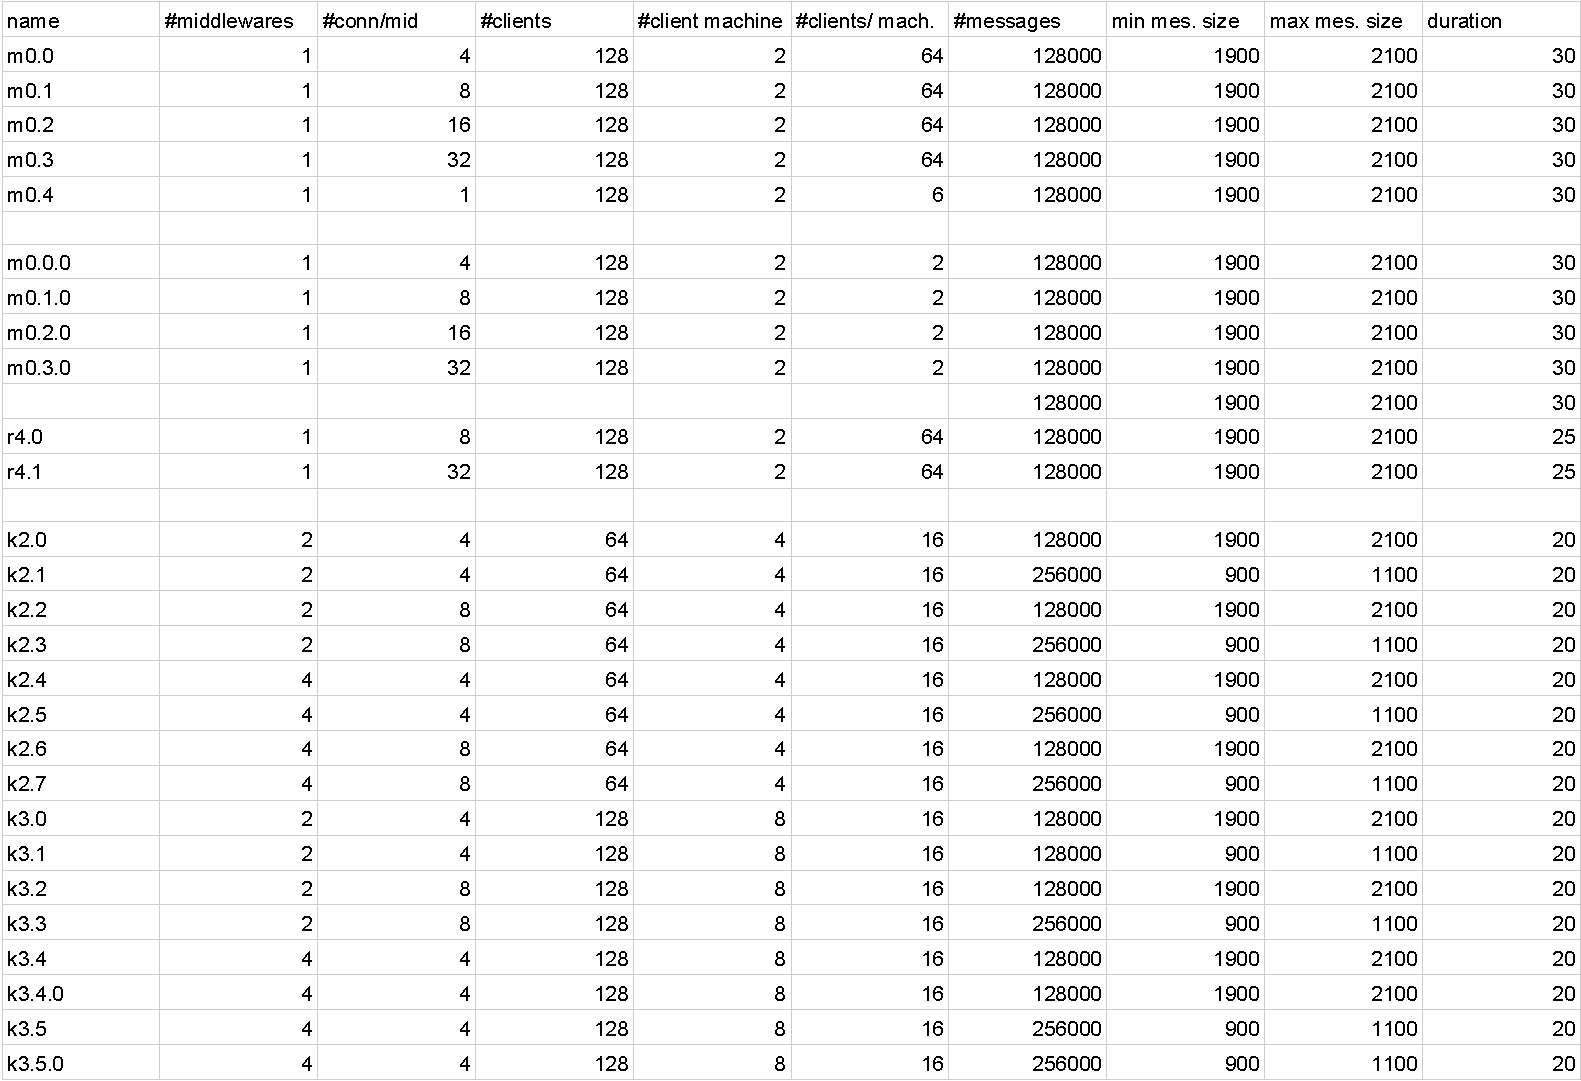
\includegraphics[scale=0.5]{exp}
\caption{Experiments Overview}
\label{fig:exp}
\end{adjustwidth}
\end{figure}


\subsection{Stability}
In this section I will show that my system runs stable. This is shown with the same experiments as the middleware testing has been done. For this section I evaluated 8 experiments, the experiments are called m0.*, where the experiments m0.0 to m0.3 describe the first run, the experiments m0.0.0 to m0.3.0 describe the second run. The two sets of experiments have been conducted on two consecutive days, but with a time difference of 6 hours.

\subsubsection{Database}
First I show that the number of messages in the database is constant over a longer period of time. This is a condition in order to get meaningful test results. This can be seen in figure \vref{fig:numDB}, where the number of messages is shown over 28 minutes from 4 different experiments. The graph shows that the number of messages fluctuates a little, but on average is always around the initial size.

\begin{figure}[H]
\centering
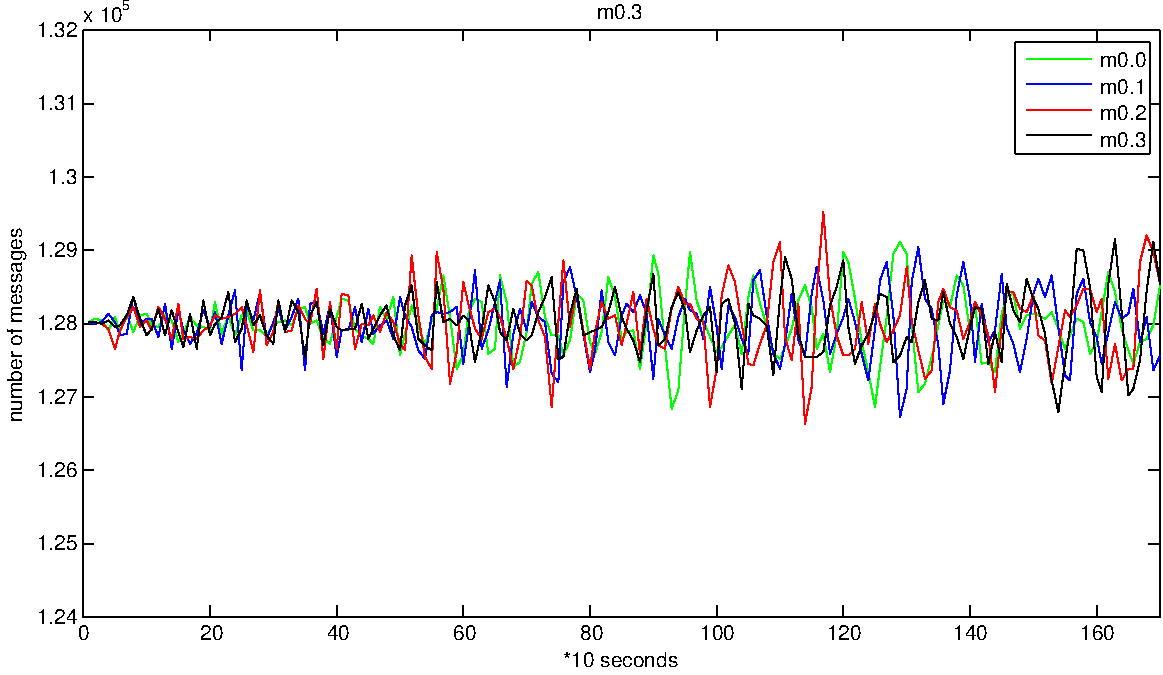
\includegraphics[scale=0.5]{mesDB}
\caption{Number of Messages in Database}
\label{fig:numDB}
\end{figure}

\begin{table}[H]

\caption{Number Of Messages in Database}
\centering
\begin{tabular}{|r|l|l|}
\toprule
Experiment & Average & StD\\
\midrule
m0.0	&	127990	&	401.1\\
m0.1 	&	127990	&	408.8\\
m0.2 	&	128000 	& 	449.6\\
m0.3 	& 	128000 	& 	402.4\\
\bottomrule
\end{tabular}
\label{tab:numb}
\end{table}

\subsubsection{Amazon Servers}
The Amazon servers produced very similar results for the different runs of the experiments. The clients throughput has been almost identical for all the experiments. Every subplot shows two experiments with identical configurations conducted at different times.
\TODO{skalen unterschiedlich}
\begin{figure}[H]
\centering
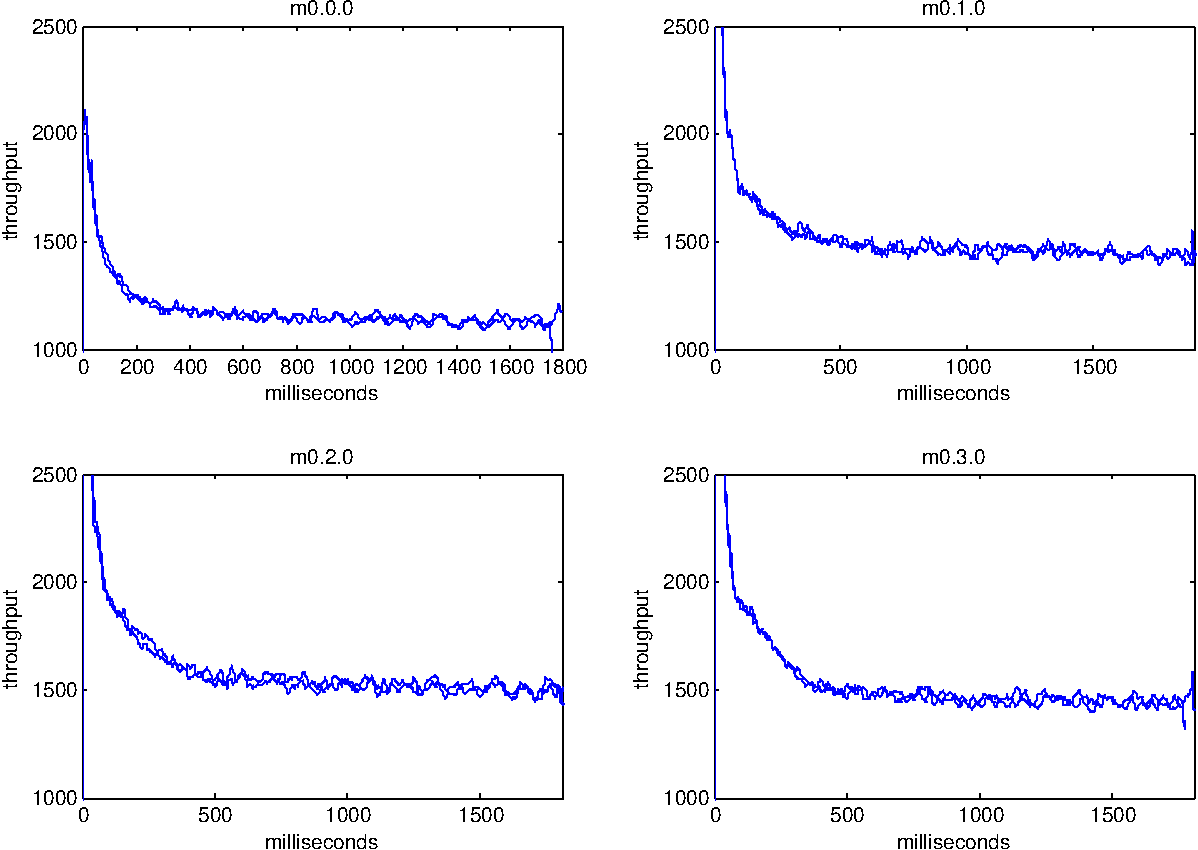
\includegraphics[scale=0.5]{midCl}
\caption{Client Throughput}
\label{fig:midCl}
\end{figure}

\subsection{Throughput and Response Time}
As can be seen in figure \vref{fig:midCl}, the throughput is very constant after a warm-up phase. I therefore did all the other experiments only over 20 minutes instead of 30. When comparing the experiments I looked at the interval from 7 to 18 minutes, since during this interval the system's performance is very stable, therefore all calculation of averages are on this interval if not stated otherwise. 
The table \vref{tab:througput} shows the similar averages for the two runs of every experiments shown in figure \vref{fig:midCl}. 

\begin{table}[H]

\caption{Client Average Throughput}
\centering
\begin{tabular}{|r|l|l|}
\toprule
Experiment & Average & StD\\
\midrule
m0.0	&	1151	&	112\\
m0.0.0 	& 	1141 	& 	101\\
m0.1 	&	1475	&	143\\
m0.1.0 	& 	1477 	& 	141\\
m0.2 	&	1537 	& 	140\\
m0.2.0 	& 	1548 	& 	139\\
m0.3 	& 	1473 	& 	129\\
m0.3.0 	& 	1477 	& 	142\\
\bottomrule
\end{tabular}
\label{tab:througput}
\end{table}

The performance drop at the beginning may have different causes. One of the causes is that the indices corrupt over time. This causes the indices and the database to grow and get slower. To show the index corruption has an effect on the throughput I conducted experiments r4.0 and r4.1. In these experiments I rebuilt the index after 15 minutes. Once with \texttt{reindex} and once with \texttt{vacuum full} which  rebuilts the database completely from the current snapshot. On the left hand side of figure \vref{fig:vacuum} one can see the database size and the effect the two operations had. On the rigt side the througput is shown. Rebuilding the database and the index clearly have a positive shortterm effect on the performance.

\begin{figure}[H]
\centering
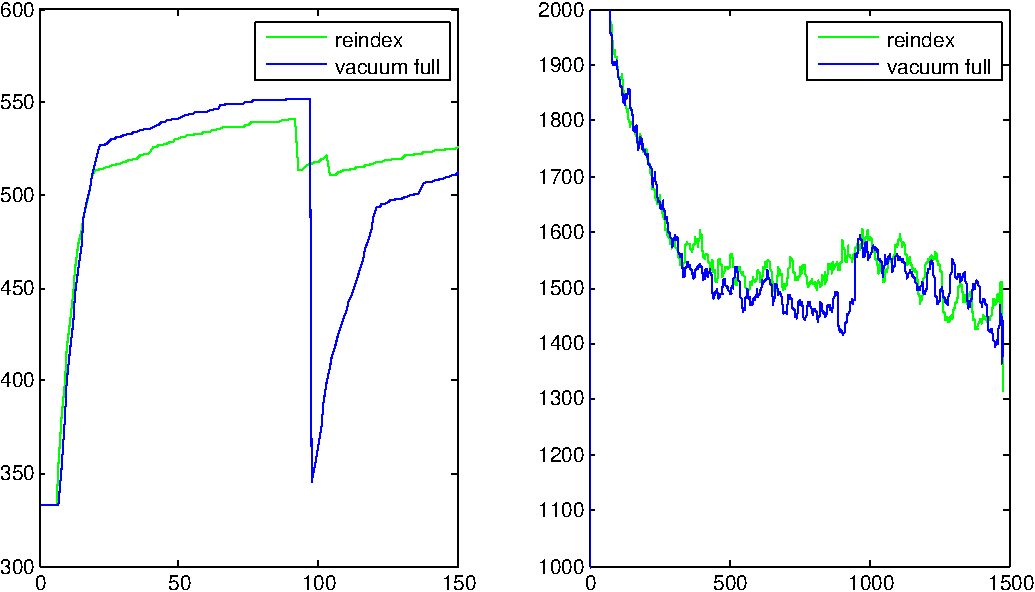
\includegraphics[scale=0.5]{vacuum}
\caption{Reindex \& Vacuum Full}
\label{fig:vacuum}
\end{figure}


\subsection{Middleware and Database in Depth}
\label{sec:middlewaretesting}
In this section I have a closer look at the system components. I therefore use the experiments m0.0.0 to m0.3.0. The idea is to show the different response times of the requests. I also compare the middleware's performance depending on how many threads and therefore database connections the middleware has. 





Figure \vref{fig:tcomp} shows that the middleware performs the poorest with 4 connections and almost identical with 8, 16 and 32 connections. This result can be expected as long as the database is not already the bottleneck with 4 connections. It can be expected because the middleware runs on a server with 8 CPU-cores and will have only half its power with 4 threads, compared to 8 or more.
 

\begin{figure}[H]
\centering
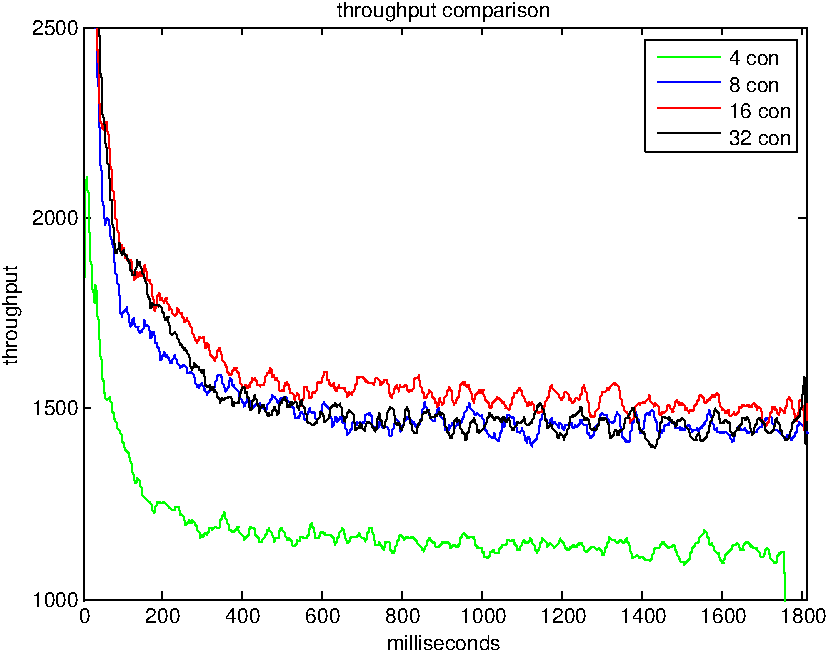
\includegraphics[scale=0.5]{tcomp}
\caption{Throughput Comparison}
\label{fig:tcomp}
\end{figure}






\subsection{System performance}
\label{sec:2k}


\begin{sidewaysfigure}[h]
\centering
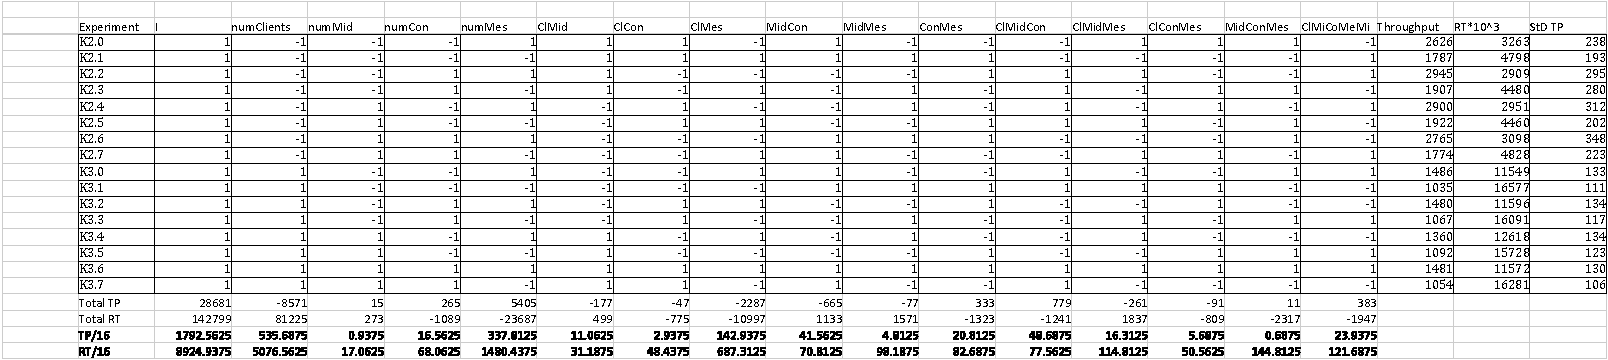
\includegraphics[scale=0.9]{2k}
\caption{2k-Tests}
\label{fig:2k}
\end{sidewaysfigure}



To evaluate the overall systems performance and to find the configuration with the highest throughput as well as to understand the relation between differnt factors I did a 2k-testing. The exact cofigurations of the 16 tests, called k\* can be found in the table \vref{fig:2k}. I selected 4 factors that I did the 2k-testing with. These factors are:
\begin{itemize}
\item number of clients
\item number of middlewares
\item number of connections per middleware
\item number of messages in the database
\end{itemize}

I decided to run 16 clients on every client server instance. I also decided to scale the number of queues in the database with the number of messages. Therefore the average number of messages in a queue is equal in all experiments. I decided to do this because when a client asks for a message in a queue, all messages in this queue have to be sorted according to the timestamp. This will take the database a long time and I wanted to test if the number of messages has an effect on the execution time and not the number of queues. I also decreased the message size for the dataset with more messages.I did this in order to reduce the effect of the database size on the performance.
Unfortunatelly I lost the statistic files of two client machine in experiment k2.3. I therefore investigated the differences of the client machines in a single experiment. Figure \vref{fig:compC} shows the 4 client machines for a single experiment in every subplot. Even in the start-up phase the different client machines behave almost equaly. I therefore conclude that doubling the data from the two client machines still gives valid results. Another indicator for the very similar performance of the client machines is given in section \vref{changes}, where I show that periodic tasks are done by all clients at almost the same time.


\begin{figure}[H]
\begin{adjustwidth}{-2in}{-2in}
\centering
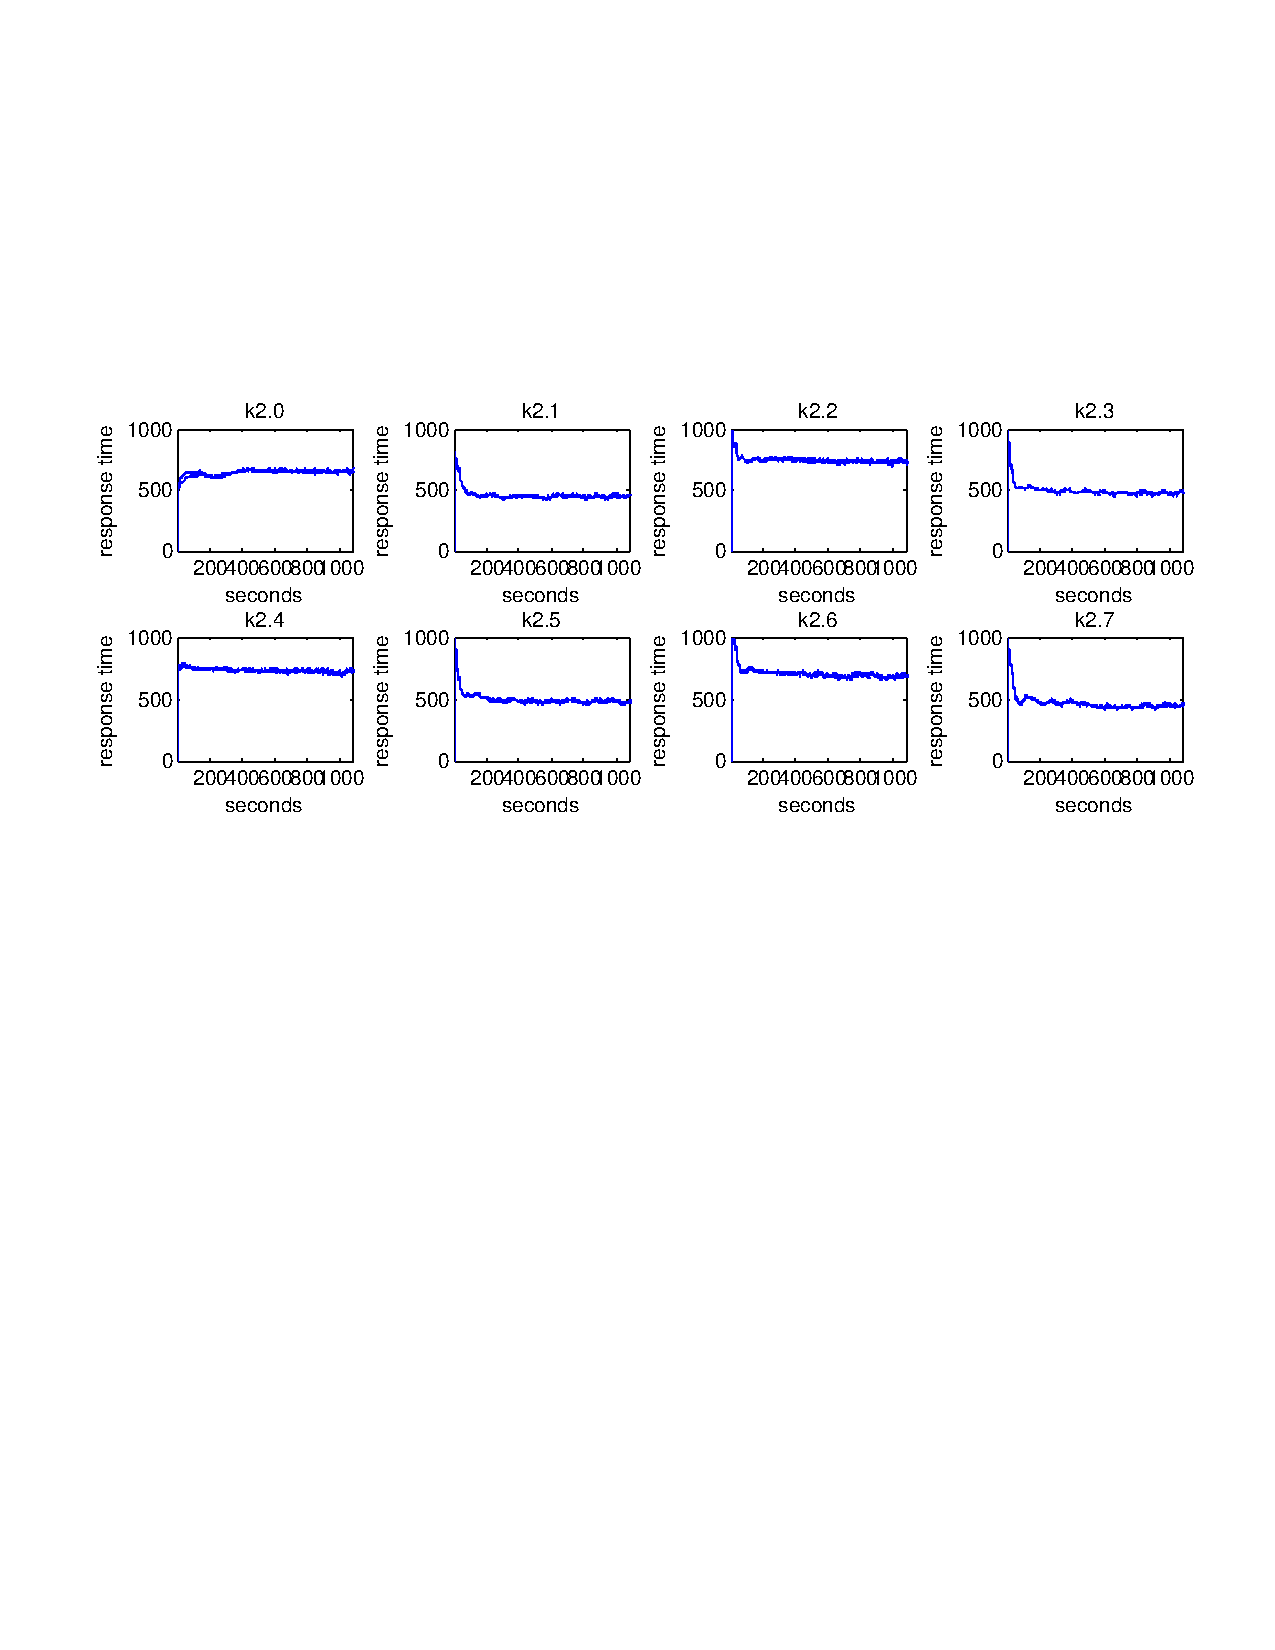
\includegraphics[scale=0.8]{compareC}
\caption{Client Machine Comparison}
\label{fig:compC}
\end{adjustwidth}
\end{figure}


The calculation of the different factors can be seen in \vref{fig:2k}. I didn't include the standard deviation for the response time. It only makes sense to include it for a single type of operation, but not for all. When a client writes to the database, the socket is close as soon as the request is given to a \texttt{Handler} thread. Therefore a write operation measures only the time in the queue, while requests with a return value measure the whole roundtrip time. Because of the very different execution times of the different requests, the standard deviation over all requests is almost as big as the average value.

The number of middlewares has little influence on the system's performance. If the number of middlewares has little influence on the system's performance than the Database has to be the bottleneck. In this case the number of connections cannot have an influence on the overall performance. This is because the database has 8 CPU-cores and should therefore perform best with 8 or 16 (hyperthreading) threads. Conducting the experiment with 8 connections per middleware would have given a performance increase in case the middleware was the bottleneck with only 4 threads, as can be seen in figure \vref{fig:tcomp}.

The number of messages has a huge impact on the system. If the database has more messages it is much slower. As already explained, this is not because the queues are longer and it takes longer to sort the messages. The effect is mainly because the metadata table is twice as big for the setup with more messages. For every request the whole table, meaning one or more indices have to be queried. Since these indices are also twice as big the performance is worse. 


The number of clients has a huge impact on the systems performance. More clients reduces the throughput and increases the response time. With twice as many clients but the same database performance it can be expected that the responstime doubles, since the throughput stays the same. But I am not sure why it has such a huge influence on the throughput. A possible explenation could be that more clients increase the probability of cache misses. With fewer clients maybe the queues for most clients could be kept in memory. 



My system performs the best in experiments k2.2 and k2.4. It is obvious from that those two perform very similarly since the only difference between the experiments is the number of middlewares. As shown above the number of middlewares has little influence on my system. In both experiments the throughput reaches about 2900 requests/second, with a response time of 29 milliseconds.

\section{Possible Project Changes}
In this section I briefly describe what I would change or do additionally if I redid the project. Some of the system components would be changed, as well as the experiment setup.
\subsection{System Changes}
\label{changes}
My \texttt{ClientWorker} periodically checks for all queues, all clients and all queues where messages for this client exist. I underestimated the robustness of Amazons servers and thought that after a short period of time, the different client machines will do this update evenly distributed over the time. As it turned out, this was never the case. In all 2k-tests, a clear clustering of these updates can be seen. If I could implement the application again I would certainly do this update at random time intervalls. An example of this clustering is given for experiment k3.7 in figure \vref{fig:cluster}

\begin{figure}[H]
\centering
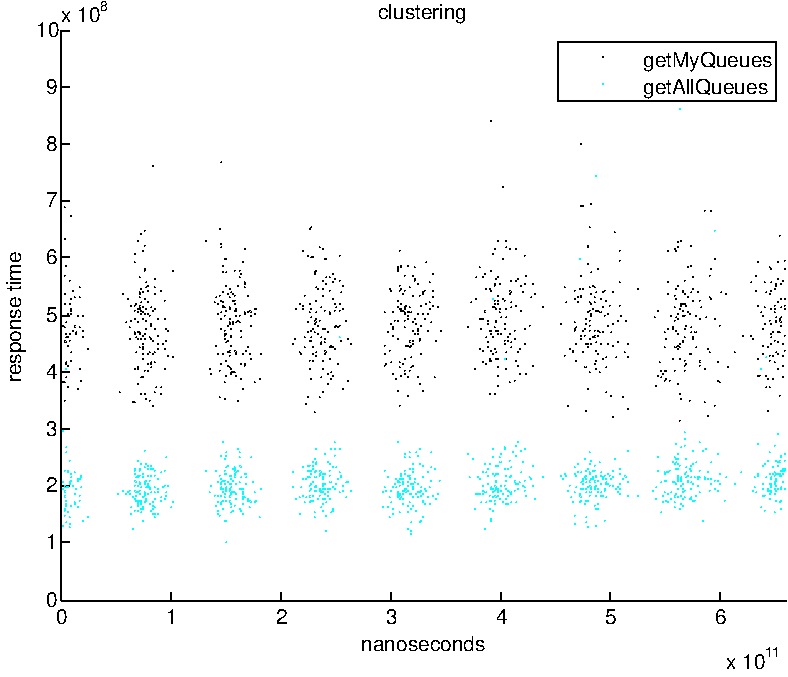
\includegraphics[scale=0.5]{cluster}
\caption{Cluster Pattern}
\label{fig:cluster}
\end{figure}


\subsection{Experiment Changes}
I explicitly didn't include the number of messages in a queue as a parameter in my tests. After seeing different behaviors of my system I wonder how the sorting of messages according to a timestamp impacts the database performance.  
The Postgres configuration also might have a huge impact on the system's performance. I only tuned a few memory and cache parameters. It would be interesting to test for the effect of these parameters. Especially the option of automatic reindexing or vacuuming would be interisting. This was not an option for this project since it could have given fluctuating throughputs. Nevertheless I think these are options that are useful in a real world system, espacially if the system runs for an extended period of time.



\end{document}